\documentclass[10pt,openany]{book}


\def\freefont{} % 使用免费商业字体
\newcommand{\mytitleen}{Typesetting Tutorial for \LaTeX}
\newcommand{\mytitle}{\LaTeX 排版教程}
\newcommand{\myauthor}{兔子草}
\newcommand{\mycp}{}

\ifdefined\freefont
    \usepackage{fontspec}
    \usepackage[fontset=none]{ctex}
    \setmainfont{EB Garamond 12 Regular}[Ligatures={Rare,Historic},Numbers=Lining,BoldFont=[EBGaramond08-Regular]]
    \setmonofont{Maple Mono Normal}

    \newfontfamily\ssfont{Vollkorn Medium Italic}
    \newfontfamily\chenfont{Vollkorn Italic}
    \newfontfamily\pagenfont{Vollkorn Italic}
    \newfontfamily\prenotefonten{EB Garamond 12 Regular}
    \newfontfamily\cpfont{Vollkorn}
    \newfontfamily\scfont{EB Garamond SmallCaps 12 Regular}

    \newfontfamily\mainreg{EB Garamond 12 Regular}[Numbers=Lining,Scale=1.2]
    \newfontfamily\mainsb{Vollkorn}[Numbers=Lining,Scale=1.15]
    \newfontfamily\mainb{Vollkorn Medium}[Scale=1.15,LetterSpace=-1]

    \newfontfamily\titlefonten{Allura}[LetterSpace=1]
    \newfontfamily\tempfont{Source Han Serif CN}

    \setCJKmainfont{Source Han Serif CN}[BoldFont=Source Han Serif CN SemiBold, ItalicFont=FZFangSong-Z02,BoldItalicFont=Source Han Serif CN Bold]
    \setCJKmonofont{FZHei-B01}

    \newCJKfontfamily\elsong{Source Han Serif CN ExtraLight}
    \newCJKfontfamily\lsong{Source Han Serif CN Light}
    \newCJKfontfamily\songti{Source Han Serif CN}
    \newCJKfontfamily\mediumsong{Source Han Serif CN Medium}
    \newCJKfontfamily\sbsong{Source Han Serif CN SemiBold}
    \newCJKfontfamily\bsong{Source Han Serif CN Bold}
    \newCJKfontfamily\hsong{Source Han Serif CN Heavy}

    \newCJKfontfamily\shusong{FZShuSong-Z01}[ItalicFont=FZKai-Z03] % 书宋
    \newCJKfontfamily\fangsong{FZFangSong-Z02} % 仿宋
    \newCJKfontfamily\heiti{FZHei-B01} % 黑体
    \newCJKfontfamily\kaiti{FZKai-Z03} % 楷体


    \newcommand{\titlefont}{\titlefonten\fangsong}
    \newcommand{\signfont}{\writing}

    \newcommand{\tocmain}{\bsong}
    \newcommand{\tocpart}{\sbsong\ssfont}
    \newcommand{\tocchapter}{\sbsong\chenfont}
    \newcommand{\tocchaplabel}{\itshape}
    \newcommand{\tocsection}{\songti}
    \newcommand{\tocsectlabel}{\scfont}
    \newcommand{\tocsubsection}{\tocsection}
    \newcommand{\tocsubsectlabel}{\tocsectlabel}
    \newcommand{\tocpage}{\pagenfont}

    \newcommand{\partfont}{\bsong\mainb}
    \newcommand{\chapterfont}{\bsong\mainb}
    \newcommand{\sectionfont}{\sbsong\mainsb}
    \newcommand{\subsectionfont}{\songti\mainreg}
    \newcommand{\pagenumberfont}{\tocpage}
    \newcommand{\headfont}{\kaiti\cpfont}
    \newcommand{\quotefont}{\itshape}
    \newcommand{\prenotefont}{\prenotefonten\sbsong}
    \newcommand{\writing}{\rmfamily\sbsong}
    \newcommand{\spellfont}{\quotefont}
    \newcommand{\dotfont}{\shusong}
\else
    \usepackage{ctex}
    \newcommand{\prenotefont}{\rmfamily}
    \newcommand{\titlefont}{}
    \newcommand{\signfont}{\ttfamily}
    \newcommand{\cpfont}{\ttfamily}

    \newcommand{\tocmain}{\bfseries}
    \newcommand{\tocpart}{\bfseries}
    \newcommand{\tocchapter}{\itshape}
    \newcommand{\tocchaplabel}{\itshape}
    \newcommand{\tocsection}{\rmfamily}
    \newcommand{\tocsectlabel}{\rmfamily}
    \newcommand{\tocsubsection}{\tocsection}
    \newcommand{\tocsubsectlabel}{\tocsectlabel}
    \newcommand{\tocpage}{\ttfamily}
    \newcommand{\ssfont}{\itshape}

    \newcommand{\partfont}{\bfseries\itshape}
    \newcommand{\chapterfont}{\bfseries}
    \newcommand{\sectionfont}{\bfseries}
    \newcommand{\subsectionfont}{\sffamily}
    \newcommand{\pagenumberfont}{\tocpage}
    \newcommand{\headfont}{\ttfamily}
    \newcommand{\quotefont}{\itshape}
    \newcommand{\writing}{\rmfamily\ttfamily}
    \newcommand{\spellfont}{\quotefont}
    \newcommand{\dotfont}{\rmfamily}
    \newcommand{\tempfont}{\rmfamily}
\fi

% 字体配置
\ifdefined\freefont
    \usepackage{fontspec}
    \usepackage[fontset=none]{ctex}
    \setmainfont{EB Garamond 12 Regular}[Ligatures={Rare,Historic},Numbers=Lining,BoldFont=[EBGaramond08-Regular]]
    \setmonofont{Maple Mono Normal}

    \newfontfamily\ssfont{Vollkorn Medium Italic}
    \newfontfamily\chenfont{Vollkorn Italic}
    \newfontfamily\pagenfont{Vollkorn Italic}
    \newfontfamily\prenotefonten{EB Garamond 12 Regular}
    \newfontfamily\cpfont{Vollkorn}
    \newfontfamily\scfont{EB Garamond SmallCaps 12 Regular}

    \newfontfamily\mainreg{EB Garamond 12 Regular}[Numbers=Lining,Scale=1.2]
    \newfontfamily\mainsb{Vollkorn}[Numbers=Lining,Scale=1.15]
    \newfontfamily\mainb{Vollkorn Medium}[Scale=1.15,LetterSpace=-1]

    \newfontfamily\titlefonten{Allura}[LetterSpace=1]
    \newfontfamily\tempfont{Source Han Serif CN}

    \setCJKmainfont{Source Han Serif CN}[BoldFont=Source Han Serif CN SemiBold, ItalicFont=FZFangSong-Z02,BoldItalicFont=Source Han Serif CN Bold]
    \setCJKmonofont{FZHei-B01}

    \newCJKfontfamily\elsong{Source Han Serif CN ExtraLight}
    \newCJKfontfamily\lsong{Source Han Serif CN Light}
    \newCJKfontfamily\songti{Source Han Serif CN}
    \newCJKfontfamily\mediumsong{Source Han Serif CN Medium}
    \newCJKfontfamily\sbsong{Source Han Serif CN SemiBold}
    \newCJKfontfamily\bsong{Source Han Serif CN Bold}
    \newCJKfontfamily\hsong{Source Han Serif CN Heavy}

    \newCJKfontfamily\shusong{FZShuSong-Z01}[ItalicFont=FZKai-Z03] % 书宋
    \newCJKfontfamily\fangsong{FZFangSong-Z02} % 仿宋
    \newCJKfontfamily\heiti{FZHei-B01} % 黑体
    \newCJKfontfamily\kaiti{FZKai-Z03} % 楷体


    \newcommand{\titlefont}{\titlefonten\fangsong}
    \newcommand{\signfont}{\writing}

    \newcommand{\tocmain}{\bsong}
    \newcommand{\tocpart}{\sbsong\ssfont}
    \newcommand{\tocchapter}{\sbsong\chenfont}
    \newcommand{\tocchaplabel}{\itshape}
    \newcommand{\tocsection}{\songti}
    \newcommand{\tocsectlabel}{\scfont}
    \newcommand{\tocsubsection}{\tocsection}
    \newcommand{\tocsubsectlabel}{\tocsectlabel}
    \newcommand{\tocpage}{\pagenfont}

    \newcommand{\partfont}{\bsong\mainb}
    \newcommand{\chapterfont}{\bsong\mainb}
    \newcommand{\sectionfont}{\sbsong\mainsb}
    \newcommand{\subsectionfont}{\songti\mainreg}
    \newcommand{\pagenumberfont}{\tocpage}
    \newcommand{\headfont}{\kaiti\cpfont}
    \newcommand{\quotefont}{\itshape}
    \newcommand{\prenotefont}{\prenotefonten\sbsong}
    \newcommand{\writing}{\rmfamily\sbsong}
    \newcommand{\spellfont}{\quotefont}
    \newcommand{\dotfont}{\shusong}
\else
    \usepackage{ctex}
    \newcommand{\prenotefont}{\rmfamily}
    \newcommand{\titlefont}{}
    \newcommand{\signfont}{\ttfamily}
    \newcommand{\cpfont}{\ttfamily}

    \newcommand{\tocmain}{\bfseries}
    \newcommand{\tocpart}{\bfseries}
    \newcommand{\tocchapter}{\itshape}
    \newcommand{\tocchaplabel}{\itshape}
    \newcommand{\tocsection}{\rmfamily}
    \newcommand{\tocsectlabel}{\rmfamily}
    \newcommand{\tocsubsection}{\tocsection}
    \newcommand{\tocsubsectlabel}{\tocsectlabel}
    \newcommand{\tocpage}{\ttfamily}
    \newcommand{\ssfont}{\itshape}

    \newcommand{\partfont}{\bfseries\itshape}
    \newcommand{\chapterfont}{\bfseries}
    \newcommand{\sectionfont}{\bfseries}
    \newcommand{\subsectionfont}{\sffamily}
    \newcommand{\pagenumberfont}{\tocpage}
    \newcommand{\headfont}{\ttfamily}
    \newcommand{\quotefont}{\itshape}
    \newcommand{\writing}{\rmfamily\ttfamily}
    \newcommand{\spellfont}{\quotefont}
    \newcommand{\dotfont}{\rmfamily}
    \newcommand{\tempfont}{\rmfamily}
\fi


% 首段缩进
\usepackage{indentfirst}

% 启用并隐藏超链接
\usepackage{hyperref}
\hypersetup{hidelinks}

% 调整行距
\usepackage{setspace}
\newcommand{\mysetspacing}{
    \setstretch{1.618}
}
\mysetspacing

% 段距
\setlength{\parskip}{0pt}

% 页面配置
\usepackage{geometry}
% 主布局
\newlength{\pw}
\newlength{\ph}
% A5 148*210
\setlength{\pw}{148mm}
\setlength{\ph}{210mm}

\newlength{\bleedlen}
\setlength{\bleedlen}{0mm}

\newlength{\ptop}
\newlength{\pbottom}
\newlength{\pinner}
\newlength{\pouter}
\newlength{\phsep}
\newlength{\pfskip}

\setlength{\ptop}{21mm}
\setlength{\pbottom}{21mm}
\setlength{\pinner}{22mm}
\setlength{\pouter}{13.5mm}
\setlength{\phsep}{.8\baselineskip}
\setlength{\pfskip}{2.2\baselineskip}
\addtolength{\pfskip}{-1em}
% 目录页布局
\newcommand{\tocgeo}{}
% 图片页布局
\newcommand{\picgeo}{\newgeometry{top=\bleedlen,bottom=\bleedlen,inner=\bleedlen,outer=\bleedlen}}
% 图片页布局
\newcommand{\buindinpicgeo}{}

\ifdefined\bleed
    \addtolength{\bleedlen}{3mm}
    \addtolength{\pw}{\bleedlen}
    \addtolength{\pw}{\bleedlen}
    \addtolength{\ph}{\bleedlen}
    \addtolength{\ph}{\bleedlen}
    \addtolength{\ptop}{\bleedlen}
    \addtolength{\pbottom}{\bleedlen}
    \addtolength{\pinner}{\bleedlen}
    \addtolength{\pouter}{\bleedlen}
    \renewcommand{\tocgeo}{\newgeometry{left=30mm,right=30mm,top=\ptop,bottom=\pbottom}}
\else
    \renewcommand{\tocgeo}{\newgeometry{left=27mm,right=27mm,top=\ptop,bottom=\pbottom}}
\fi

\newcommand{\charcount}{32}
\newcommand{\linecount}{25}

\newlength{\theight}
\setlength{\theight}{\linecount\baselineskip}
\addtolength{\theight}{1em}
\addtolength{\theight}{-\baselineskip}

\geometry{
    paperwidth=\pw,
    paperheight=\ph,
    top=\ptop,
    outer=\pouter,
    % inner=\pinner,
    % bottom=\pbottom,
    textwidth=\charcount\ccwd,
    textheight=\theight,
    headsep=\phsep,
    footskip=\pfskip
}

% 空白页
\newcommand{\blankpage}{
    \newpage
    \makebox{}
    \thispagestyle{empty}
    \newpage
}

% 空白段
\newcommand{\blankpar}{
    ~\
}

% 目录
% 目录参数
\counterwithout{section}{chapter}
\counterwithout{subsection}{section}
% 目录格式
\usepackage{titletoc}
% 章节符号
\newcommand{\myss}{\ssfont\S}
% 目录标题
\renewcommand{\contentsname}{
    目\quad 录
}
% 目录内标题格式
\titlecontents{part}
[0em]
{\vspace{1em}\Large\tocpart}
{}
{}
{\hspace{4mm}\pagenumberfont\contentspage}[\vspace{0.5em}]

\titlecontents{chapter}
[6mm]
{\vspace{0.3em}\large\tocchapter}
{\makebox[10mm][l]{\myss\hspace{0.1em}\normalsize\uppercase\expandafter{\romannumeral\thecontentslabel}}}
{}
{\hspace{4mm}\tocpage\large\contentspage}[\vspace{0.3em}]

\titlecontents{section}
[12mm]
{\tocsection}
{\tocsectlabel Ch \hspace{0.1em}\makebox[1em][c]{\thecontentslabel}\hspace{1em}}{}
{\hspace{5mm}\tocpage\contentspage}[\vspace{0.1em}]

\makeatletter
% 页码宽度
\renewcommand{\contentspage}[1][\thecontentspage]{\hb@xt@\@pnumwidth{#1\hfil}}
\renewcommand{\@pnumwidth}{9mm}
% 每章重置尾注编号
\@addtoreset{endnote}{chapter}  % Reset endnote numbering every new chapter
\@addtoreset{subsection}{section} % Reset subsection numbering every new section
\@addtoreset{section}{chapter} % Reset section numbering every new chapter
\@addtoreset{chapter}{part}  % Reset chapter numbering every new part
\makeatother
% 每页重置脚注编号
\usepackage{footnpag}

% 正文标题格式
\usepackage{titlesec}

\titleformat{\part}[display]{\centering\huge\partfont}{\thepart}{1.5pc}{\thispagestyle{empty}}
\titlespacing{\part}{0em}{.3\textheight}{0em}

\titleformat{\chapter}{\centering\Large\chapterfont}{}{0em}{}
\titlespacing{\chapter}{0em}{.5\baselineskip}{2\baselineskip}

\titleformat{\section}{\sectionfont}{Chapter~\thesection}{1em}{}
\titlespacing{\section}{2em}{1.4\baselineskip plus 2pt minus 2pt}{.5\baselineskip plus 2pt minus 2pt}

\titleformat{\subsection}{\subsectionfont}{0\thesubsection}{1em}{}
\titlespacing{\subsection}{2em}{.5\baselineskip plus 2pt minus 2pt}{.5\baselineskip plus 2pt minus 2pt}

\newcommand{\parttitle}{部名}

\usepackage{fancyhdr}
% 章节标记不出现chapter和序号
\renewcommand{\chaptermark}[1]{\markboth{\MakeUppercase{#1}}{}}
\renewcommand{\sectionmark}[1]{\markright{#1}}
% 去除页眉横线
\renewcommand{\headrulewidth}{0pt}
% 页脚溢出一点
\fancyfootoffset[RO,LE]{1.5em}
\fancypagestyle{mystyle}{
    \fancyhf{}
    \fancyhead[CE]{\headfont\mytitle}
    \fancyhead[CO]{\headfont\parttitle}
    \fancyfoot[CO]{\hfill\headfont\leftmark\qquad\rule[-4pt]{0.3pt}{20pt}\hspace{1.5em}}
    \fancyfoot[RO]{\pagenumberfont\thepage}
    \fancyfoot[LE]{\pagenumberfont\thepage}
    \fancyfoot[CE]{\hspace{1.5em}\rule[-4pt]{0.3pt}{20pt}\qquad\headfont\parttitle\hfill}
}
\fancypagestyle{plain}{
    \fancyhf{}
    \fancyfoot[CO]{\hfill\headfont\leftmark\qquad\rule[-4pt]{0.3pt}{20pt}\hspace{1.5em}}
    \fancyfoot[RO]{\pagenumberfont\thepage}
    \fancyfoot[LE]{\pagenumberfont\thepage}
    \fancyfoot[CE]{\hspace{1.5em}\rule[-4pt]{0.3pt}{20pt}\qquad\headfont\parttitle\hfill}
}
\usepackage{emptypage}

% 尾注
\usepackage{endnotes}
\renewcommand{\notesname}{注:}
\renewcommand{\enoteheading}{\section*{\notesname}\mbox{}\par\vskip-\baselineskip}
\renewcommand{\theendnote}{\roman{endnote}}

% 以下为非通用内容

% 故事完
\newcommand{\storyend}[1][完]{
    \vspace{1.5\baselineskip}

    \blankpar

    \hfill \textbf{#1} \hspace{5em}

    \vspace{2\baselineskip}

    \vfill
}

\usepackage{changepage}
\renewenvironment{quotation}{
    \begin{adjustwidth}{2em}{2em}
        \quotefont
        }{
    \end{adjustwidth}
    \vspace{.5\baselineskip plus .5\baselineskip}
}
\renewenvironment{quote}{
    \vspace{0pt plus .3\baselineskip}

    \begin{adjustwidth}{2em}{2em}
        \quotefont}{
    \end{adjustwidth}

    \vspace{.3\baselineskip}
}


% 设置署名
\newcommand{\signature}{
    \vfill
    \setstretch{1.5}

    \begin{figure}[h]
        \hfill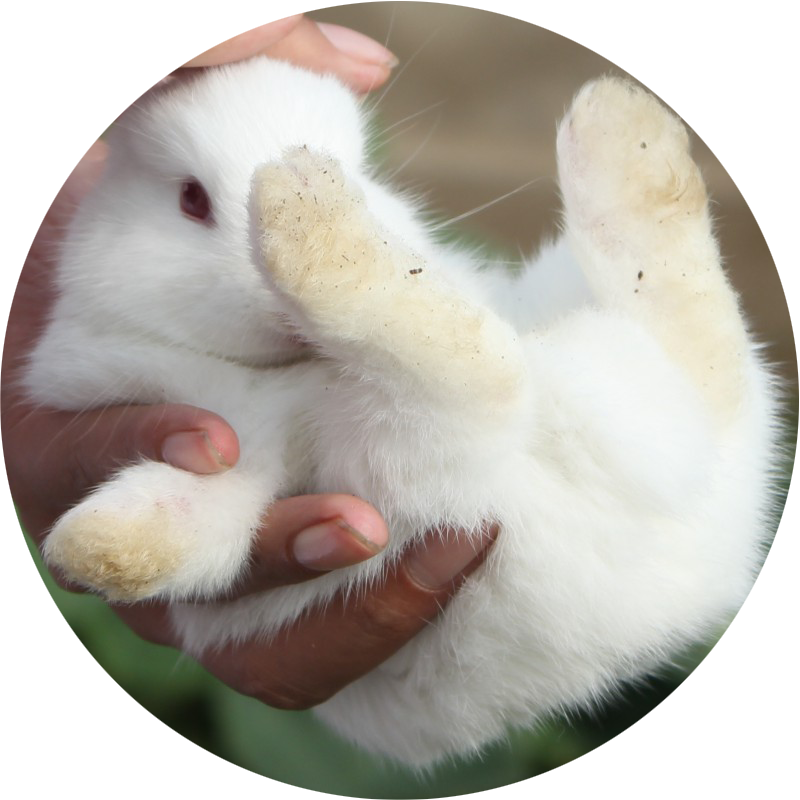
\includegraphics[width=2.8em]{headshot.png}\hspace{5.1em}
    \end{figure}

    \vspace{-1.5em}

    \hfill {\subsectionfont by\myauthor}\hspace{5em}

    \hfill {\subsectionfont \number\year.\number\month.\number\day} \hspace{4.8em}

    \vspace{2cm}
}

% 特殊符号和字体
\newcommand{\splitdot}{\dotfont ·}

\newcommand{\spell}[1]{{\spellfont #1}}

\newcommand{\tempsymbol}{{\tempfont℃}}

\newcommand{\chsline}{\makebox[2em]{——}}

% 章前注
\newcommand{\prenotes}[1]{
    \vspace{2em}
    {\prenotefont #1}
    % #1
    \vspace{0.5em}
}
% 章前注的参数
\newlength{\chapterblank}
\setlength{\chapterblank}{3cm}
\newlength{\prenoteblank}
\setlength{\prenoteblank}{3em}
\newcommand{\doublelinechapter}{{\huge\vspace{-\baselineskip}}}

% 扉页
\newcommand{\mytitlepage}{
    \null
    \vfill
    \thispagestyle{empty}

    \begin{center}
        \Huge

        \titlefont

        {\mytitleen}

        \vspace{2mm}

        {\mytitle}

        \Large

        \vspace{60mm}

        {\cpfont\mycp}

        \vspace{2mm}

        {\signfont BY \myauthor}
    \end{center}

    \vfill

    \clearpage
}

% 尾页
\newcommand{\myendpage}{
    \newpage
    \ifodd\thepage
        \blankpage
    \fi

    \newpage

    \thispagestyle{empty}

    \

    \vfill

    \begin{minipage}{50mm}

        模板制作:兔子草

    \end{minipage}
    \vspace{5mm}
}

% 插入图片
\usepackage{graphicx}

% 让脚注不影响上文的行距
\usepackage[bottom]{footmisc}
% 脚注上方高度
\setlength{\footnotesep}{8pt}
% 脚注上方横线
\renewcommand{\footnoterule}{
    \kern -2pt
    \hrule width .25\textwidth height 0.5pt
    \kern 1.5pt
}

% section上方弹性换页
\usepackage{needspace}
\AddToHook{cmd/section/before}{\needspace{3\baselineskip}}

\let\origpart\part
\renewcommand*{\part}[2][]{
    \ifx\\#1\\% optional argument not present?
    \origpart{#2}
        \renewcommand*\parttitle{#2}
    \else
    \origpart[#1]{#2}
        \renewcommand*\parttitle{#1}
    \fi
    \mysetspacing
}


% 这部分设定纯为教程服务 
\usepackage{xcolor}
\definecolor{gray}{RGB}{68,71,90}
\definecolor{grayblue}{RGB}{98,144,164}
\definecolor{cyan}{RGB}{139, 233, 253}
\definecolor{green}{RGB}{80, 250, 123}
\definecolor{orange}{RGB}{255, 184, 108}
\definecolor{pink}{RGB}{255, 121, 198}
\definecolor{purple}{RGB}{189, 147, 249}
\definecolor{red}{RGB}{255, 85, 85}
\definecolor{yellow}{RGB}{241, 250, 140}
\definecolor{myblack}{RGB}{32, 34, 39}
\definecolor{darkgreen}{RGB}{31,138,35}
\hypersetup{colorlinks,linkcolor=black,urlcolor=darkgreen}
\usepackage{metalogo}
\setmonofont{Inconsolata}
\setCJKmonofont{FZHei-B01}
\usepackage{enumitem}
\usepackage{ulem}
\usepackage{listings}
\renewcommand{\lstlistingname}{代码}
\renewcommand{\lstlistlistingname}{代码}
\lstset{
    flexiblecolumns,
    numbers=left,
    numberstyle=\footnotesize\color{gray},
    frame=leftline,
    showspaces=false,
    linewidth=\linewidth,
    xleftmargin=2\ccwd,
    breaklines=true,
    columns=fixed,
    basicstyle=\small\ttfamily,
    captionpos=b,
}
\lstdefinestyle{TeX}{
    language=TeX,
    morekeywords={usepackage,begin,newcommand,renewcommand,counterwithout,setcounter,addcounter,part,chapter,section,clearpage,newpage,cleardoublepage,thepage,setlength,addtolength,newlength,ctexset,plus,minus,makeatletter,makeatother,patchcmd,@addtoreset,addcontentsline},
    emph={documentclass,document,setmainfont,newfontfamily,BoldFont,ItalicFont,setCJKmainfont,newCJKfontfamily,geometry,newgeometry,restoregeometry,titleformat,titlespacing,blankpage,singlespacing,onehalfspacing,doublespacing,setstretch,pagestyle,thispagestyle,punctstyle,roman,titlecontents,vspace,hspace,makebox,mbox,@pnumwidth,startcontents,stopcontents,printcontents,hypersetup,fancypagestyle,fancyhf,fancyhead,fancyfoot,markboth,markright,fancyhfoffset,fancyheadoffset,fancyfootoffset,includegraphics,figure,caption,captionsetup,includepdf,subfile},
    basicstyle=\small\ttfamily\color{myblack},
    identifierstyle=\color{purple},
    keywordstyle=\color{pink},
    emphstyle=\color{orange},
    stringstyle=\color{yellow},
    commentstyle=\color{grayblue},
}
\usepackage{makecell}
\newcommand{\emoji}[1]{\fontspec{Symbola}\symbol{#1}}
\newcommand{\checkmark}{
    \makebox[1\ccwd]{
        \fboxsep1.5pt
        \colorbox{green}{\emoji{"2714}}
    }
}
\usepackage{longtable}
\newenvironment{tightitem}
{\begin{itemize}[topsep=0pt,partopsep=0pt,itemsep=0pt,parsep=0pt,leftmargin=3\ccwd,labelwidth=1.5\ccwd,labelsep=.5\ccwd]}
        {\end{itemize}}

\newenvironment{tightenum}
{\begin{enumerate}[topsep=0pt,partopsep=0pt,itemsep=0pt,parsep=0pt,leftmargin=3\ccwd,labelwidth=1.5\ccwd,labelsep=.5\ccwd]}
        {\end{enumerate}}

\newcommand{\testtext}{

    发情期的Alpha小红咬住Omega小明的腺体,开始默数30秒。}
\usepackage{float}
\fancypagestyle{mystyle}{
    \fancyhf{}
    \fancyhead[CE]{\headfont\mytitle}
    \fancyhead[CO]{\headfont BY \myauthor}
    \fancyfoot[CO]{\hfill\headfont\leftmark\qquad\rule[-4pt]{0.3pt}{20pt}\hspace{1.5em}}
    \fancyfoot[RO]{\pagenumberfont\thepage}
    \fancyfoot[LE]{\pagenumberfont\thepage}
    \fancyfoot[CE]{\hspace{1.5em}\rule[-4pt]{0.3pt}{20pt}\qquad\headfont\uppercase\expandafter{\romannumeral\thechapter}\hfill}
}
\fancypagestyle{plain}{
    \fancyhf{}
    \fancyfoot[CO]{\hfill\headfont\leftmark\qquad\rule[-4pt]{0.3pt}{20pt}\hspace{1.5em}}
    \fancyfoot[RO]{\pagenumberfont\thepage}
    \fancyfoot[LE]{\pagenumberfont\thepage}
    \fancyfoot[CE]{\hspace{1.5em}\rule[-4pt]{0.3pt}{20pt}\qquad\headfont\uppercase\expandafter{\romannumeral\thechapter}\hfill}
}

\renewcommand{\charcount}{40}
\renewcommand{\linecount}{32}

\setlength{\theight}{\linecount\baselineskip}
\addtolength{\theight}{1em}
\addtolength{\theight}{-\baselineskip}

\geometry{
    paperwidth=6.625in,
    paperheight=10.25in,
    top=\ptop,
    outer=\pouter,
    % inner=\pinner,
    % bottom=\pbottom,
    textwidth=\charcount\ccwd,
    textheight=\theight,
    headsep=\phsep,
    footskip=\pfskip,
}

\setstretch{1.3}

\titlecontents{chapter}
[6mm]
{\vspace{0.3em}\large\tocchapter}
{\makebox[10mm][l]{\normalsize\uppercase\expandafter{\romannumeral\thecontentslabel}}}
{}
{\hspace{4mm}\tocpage\large\contentspage}[\vspace{0.3em}]

\titlecontents{section}
[12mm]
{\tocsection}
{\tocsectlabel \S \hspace{0.1em}\makebox[1.2em][c]{\thecontentslabel}\hspace{1em}}{}
{\hspace{5mm}\tocpage\contentspage}[\vspace{0.1em}]

\titlecontents{subsection}
[18mm]
{\tocsubsection}
{\small\tocsubsectlabel\hspace{0.2em}\makebox[1em][c]{\thecontentslabel}\hspace{0.8em}}{}
{\hspace{7mm}\small\tocpage\contentspage}{}

\titleformat{\chapter}{\centering\Large\chapterfont}{\uppercase\expandafter{\romannumeral\thechapter}}{1em}{}
\titleformat{\section}{\sectionfont}{\S~\thesection}{1em}{}


\begin{document}

\pagenumbering{roman}

\pagestyle{mystyle}

\startcontents[tutorial]

\mytitlepage

\null\vfill

本文为懂得\LaTeX 基础命令、语法,准备以此为排版工具,制作\textbf{书籍类同人本}的玩家撰写。考虑了等宽文字与不等宽文字(通常就是中英文)掺杂的情况。有少量场景与操作系统有关,本文暂只有Windows的解决方案。

其中不包含\LaTeX 安装等入门内容。这部分教程在网上已经很多,不需要我再抄一遍。

我创立了一个模板,欢迎直接\href{https://github.com/zhuty18/fanfiction-sample}{下载使用\footnote{https://github.com/zhuty18/fanfiction-sample}}。如果本文或者本模板对你出本有帮助,你出本时感谢我一下也挺好的。(我的ID是兔子草)

本教程包含一些高投入低回报的内容,标注了“(进阶)”的字样。

\vfill\vfill

\tableofcontents

\cleardoublepage

\setcounter{page}{1}
\pagenumbering{arabic}

\chapter{\LaTeX 的优点}

一般我们看到讲\LaTeX 的文章,总难免骂两句这东西磨磨唧唧的渲染、乱七八糟的规范和屎山一样的包。正因如此,无数人试图取代\LaTeX ,但它目前依然是唯一可靠的学术类排版工具,也是世界上最流行的排版系统之一,这足以证明它的独特价值。

或许这句话有点反直觉,但是外行人想要排出一个“\textbf{能看的印刷品}”,\LaTeX 是最快也最简单的解决方案。

\section{简单易上手}

\href{https://cn.overleaf.com/}{\textit{Overleaf}\footnote{https://cn.overleaf.com/}}是\LaTeX 的在线IDE,全网页端,只需注册一个账号就可免费使用。在工作区左侧先点击目录(Menu),将编译引擎换成\XeLaTeX(\texttt{XeLaTeX})或\LuaLaTeX(\texttt{LuaLaTeX}),才可正常处理中文。拼写检查系统不支持中文,建议关掉,不然中文全篇都是拼写警告。

截止到写这篇文档的\today,\textit{Overleaf}为免费用户提供20秒的编译时间,不放图绝对够用了。(编译一个370页,20万字的本大概需要10秒)。

不过,如果想自定义字体的话,\textit{Overleaf}无能为力,还是需要自己安装\textit{TeXLive}\footnote{\textit{TeXLive}:\LaTeX 的编译器,仅能通过命令行使用,建议搭配\textit{VSCode}或\textit{TeXstudio}等工具。},在本地进行工作。

我的模板传到了\textit{Overleaf}上,但是公开模板需要等待审核检查,等通过了我会在这里放出链接。

\section{纯粹的排版工具}

目前的DIY出本教程里面,排版这一步都是用\textit{InDesign}。但\textit{InDesign}本质上是\textbf{版式设计}软件,面向市场是杂志、画册、报纸等类型。目标情景是一页上要分若干区,有的区填字、有的区放图,设计者主要研究这些区域如何分配面积、如何摆放、如何提升信息传达率、如何保持美观。

那么问题来了,\emph{你真的需要这些功能吗?}还是说,其实你需要的只是一个“能把我想印的那点东西\textbf{漂亮又简单地打包成印刷用pdf}”的工具呢?

\LaTeX 是一个简单粗暴的排版软件。格式越简单、越统一,用它来做就越容易。

排个书、插个图、把一页页画好的漫画封装成指定纸张大小的pdf……放在设计业内属于绝对的轻度需求,而\TeX 就是为这些轻度需求而生的。它的目的不是把二十页纸排出花来,而是\textbf{让八百页的文档看源文件就知道格式不会出错。}

\section{创作与排版的分离}

\LaTeX 里,创作和排版天然分离,十分契合同人创作的规律。

出同人本,无一例外是拿着内容补格式。同人文的传播载体是朴实无华的txt,偶有文画双修的大佬,也基本都是图文分离式发放。这样的创作基础天然就适配\LaTeX 。

\LaTeX 的使用步骤分为两步,先用文本编辑器撰写工作文件,再用引擎编译出结果pdf。在已有内容的情况下,只需要给内容文件增加简单的标记(基本也就是各级标题,有些作者会有脚注尾注,最多再有加粗斜体),通过简单的代码结构设计实现文档内容与格式的解耦,就能令工作空间简化且专注,只需关注排版的各项参数。

它有一点尤为可贵:手持一份十万字的文稿,正常人的直觉就是把它一次排完,然后对着pdf挑问题一个点一个点修。而排版工具里,只有\LaTeX 在一排几百页的时候不会挑你的机能。它只会慢,但不会崩。

\section{编辑与渲染的分离}

排版的本质是把文档变成一堆矢量图。这个步骤中最本质的是编辑(设定格式即转化规则),而最耗时的是渲染。

作为一个没有图形化操作界面的排版工具,\LaTeX 渲染时可以把所有资源全部用在“得到pdf”这一件事上,效率极高。如果你嫌Windows还是太慢,可以装一个WSL,再提一波生产力。

\section{默认细节极佳}

如果找一些专业的中文排版攻略读(比如\href{https://www.w3.org/TR/clreq/}{中文排版需求\footnote{https://www.w3.org/TR/clreq/}},\href{https://www.thetype.com/2020/01/16565/}{中文排版网格系统的五大迷思\footnote{https://www.thetype.com/2020/01/16565/}}),那么就会意识到,文字排版这件事其实非常细碎繁杂,需要关注的细节极多。

由于开源的特性,\LaTeX 内有着大量前人造好的轮子,可以覆盖排版时应当处理的普适性专业细节,极大地节约工作成本。用户只需要进行自己的个性化即可。对于中文,最显著的案例就是标点压缩和字距。

\begin{tightitem}
    \item 标点压缩\\在正式的排版原则中,使用全角标点时标点的宽度是会变的。较为常见的几个状态如下
    \begin{tightenum}
        \item 独立标点为1个字符宽
        \item 连续的两个标点(如\texttt{:“})合并挤压为1.5个字符宽
        \item 段首的起始标点(如\texttt{“}、\texttt{《}等)为0.5个字符宽
    \end{tightenum}
    \item 字距\\字距指文字之间的水平间距。一份理想的中文文本,应该满足以下条件:
    \begin{tightenum}
        \item 行宽可以规定
        \item 文字每行左右均顶格,恰好占满设定的行宽
        \item 当汉字与外语字符/阿拉伯数字相邻时,间距一个空格宽
        \item 在没有干扰的情况下,文字竖对齐。主要是最后一行,如果前文的字距不为默认值,那么最后一行的字距应与前文相同,而非简单左靠
    \end{tightenum}
\end{tightitem}

这些细碎的设定,在\LaTeX 的\texttt{ctex}包中默认就会满足。不需要自己进行任何选择或调整\texttt{ctex}包默认就提供最美观的排版。(破折号略有些问题,我在后文里附了解决方案)

字母类文字排版时会遇到的关键问题是,一行文字几乎不可能在换行处恰好断开。\TeX 对此的默认处理方案可谓是视觉上最美观的。\textit{Knuth-Plass}算法通过断字和拉伸,使得一段文本每行左右两侧都能对齐,且肉眼基本无法看出每行空格宽度的区别。

正因有如此基础,\LaTeX 处理混合文本时的便捷程度天下无双。

\section{一句忠告}

\LaTeX 是非常容易催生强迫症的,\emph{\textbf{千万不要追求完美}}。谨记,我们做的是同人本。

\chapter{排版参数}

\section{小说}

版式设计是为了优化信息的传达。对于小说,最重要的信息永远是故事本身,即文字内容。因此,没有必要太深入地研究版面设计。但完全不管也不行,“易读性”和“可读性”是必须要考虑的。

易读性即Legibility,对每个基础单元(中文的字、英文的单词)的识别程度,更多地指向字体。可读性即Readability,即阅读体验的舒适性。在排版中,可读性代表一段文本的阅读容易度,主要指向基础单元的排布方式,例如字距、行高。

这都是排印学里非常根本的课题。有太多的人已经研究过了,我们可以直接使用现成的结论:

行高:中文的行高一般至少是字高的1.5--1.8倍,具体数值受字体和字号的双重影响。如果行高不足,汉字等高的特性会使得行与行之间空隙不清晰,降低阅读流畅性。

行数:翻页的频次主要是行数决定的,这个数极大地影响阅读体验。对于A5大小的纸张,可以以25为参照,每页行数小于等于25时,阅读体验比较休闲,反之行数越多,越接近于专业性强的书籍,阅读体验越严肃。实际使用中,23-27行适用于小说类文章排版。

单行字数:A5这个纸张大小还没有充分利用人眼的视野空间,因此单行字数只受限于字体大小和文字区域的宽度,不需要考虑人眼阅读能力而额外分栏。通常的书籍是每行28--30个字,实际体验上,26--32都是可接受的。

\blankpar

具体选择什么样的参数,建议按自己的需求来决定。决定一个本子气质的是单页信息量(可以简单用行数*单行字数来量化)。同字号下,单页信息量越大,阅读体验越严肃;越小体验越活泼。比方说,一行18个字,2倍行高就可以轻松打造移动端的阅读体验。

但请注意,\textbf{排版越疏松,本子越厚}。\emph{\textbf{本子越厚,成本越高}}。印厂算钱的时候只看页数,不看油墨密度,页数越多就越贵。并且,对于字数较多的本,不紧凑一点真的会印成砖头的。

一个更直观的算法:\texttt{每页行数*每行字数}得到\texttt{理论每页字数},是一页纸理论上能印的字数,但实际上不可能印满(出版物上标注的字数是版面字数,约等于理论字数乘页数,所以给人的感觉很注水)。理论值乘上\texttt{0.6\textasciitilde{}0.65}才是实际上的\texttt{平均每页字数}。整个本的字数除以\texttt{平均每页字数}可以得到大约的正文页数(排版增加的留白已经考虑在内)。最通用的80g纸,厚度是0.11毫米。

所以用\texttt{总字数/每页行数/每行字数/11.364}就可以得到一个大约的厚度(单位为毫米)。

\section{全网格化(进阶)}

在正式出版物中,还有其他\sout{强迫症发作的}进阶规则。

\begin{tightenum}
    \item   行宽是整数个字的宽\\即一排汉字能将一行恰好排满,提升每页纸上的网格感。
    \item   标题所占高度是整数个行的高\\使得不同页面格式中,正文都能实现跨页行对齐。
\end{tightenum}

这些规则本质上都是令阅读体验更接近于排字印刷时代,但是到了现代,出版社也不是一定遵守这些规矩,姑且看看,了解一下即可。除非有很强的强迫症,不然不需要应用。

\begin{center}\rule{0.5\linewidth}{0.5pt}\end{center}

了解了以上内容后,就让我们进入正题,开始使用\LaTeX 进行排版。

\chapter{字体设定}

\section{字体入门}

\subsection{字体类别}

字体可以简单分为有衬线(Serif)和无衬线(Sans Serif,或简称为Sans)两类。衬线指的是笔画边角处的装饰,例如宋体是典型的衬线字体,而黑体是典型的无衬线字体。

纸张上,有衬线的字体易读性更佳,一般用于正文中;无衬线字体更加醒目,可以用于标题。

等宽字体(mono)指所有字母和符号都占据同样宽度的字体。对于中文等符号文字没有意义,咱天然就是等宽字体。对字母文字而言,等宽的易读性并不太好,应用场景很有限。除了故意模仿打字机的文字质感外,只有编程为了竖对齐使用等宽字体。

\subsection{字体风格}

一个字体名是一个系列,其中往往有多个风格,最重要的是各种字重和斜体。

字重:描述一个笔画有多粗。

从轻到重(从细到粗)分别有:thin,extra light,light,regular (normal),medium,semi bold,bold,heavy (black)。一个字体必然有字重关键词,留空时会自动使用regular。原则上的加粗行为就是字重从regular变成bold。如果一个字体没有bold字重,word还会用算法生成一种伪粗体。

斜体:Italic,严格上来说应该叫意大利体。字母文字排版时产生的风格化方案,\textbf{中文其实没有斜体},承担类似功能的是楷体或仿宋。

不是所有字体都有意大利体,很多时候我们看到的也是算法计算的伪意大利体。方案是简单将字符拉斜一些,不涉及意大利体中常见的字形变化。这种伪意大利体其实才该叫斜体(Slanted)。但由于这些风格本身的舶来性,加之Slanted几乎没什么专门的用处,大家已经习惯将Italic称作斜体,因此我后文也沿用这种通俗的误称。

\section{\texttt{ctex}包介绍}

\LaTeX 需要\texttt{ctex}包来处理中文,需要\texttt{xelatex}或\texttt{lualatex}引擎才能编译。使用方法为

\lstinputlisting[style=TeX,caption=使用\texttt{ctex}]{codes/ctex.tex}

方案一相当于建立中文文档,方案二相当于在英文文档里使用中文。方案一自动将所有预设词翻译为了中文,更加便捷;方案二在细节上更加通用。例如,按方案一生成的目录中,标题内“第x章”\,“第x部分”等字样需要用\texttt{\textbackslash{}ctexset}命令来调整;而方案二可以用更加基础(i.e.与其他包兼容性更好)的方式对这些地方进行自定义。

\texttt{ctex}包默认根据\textbf{当前操作系统}选择字体配置,策略如下

\begin{figure}[H]
    \centering
    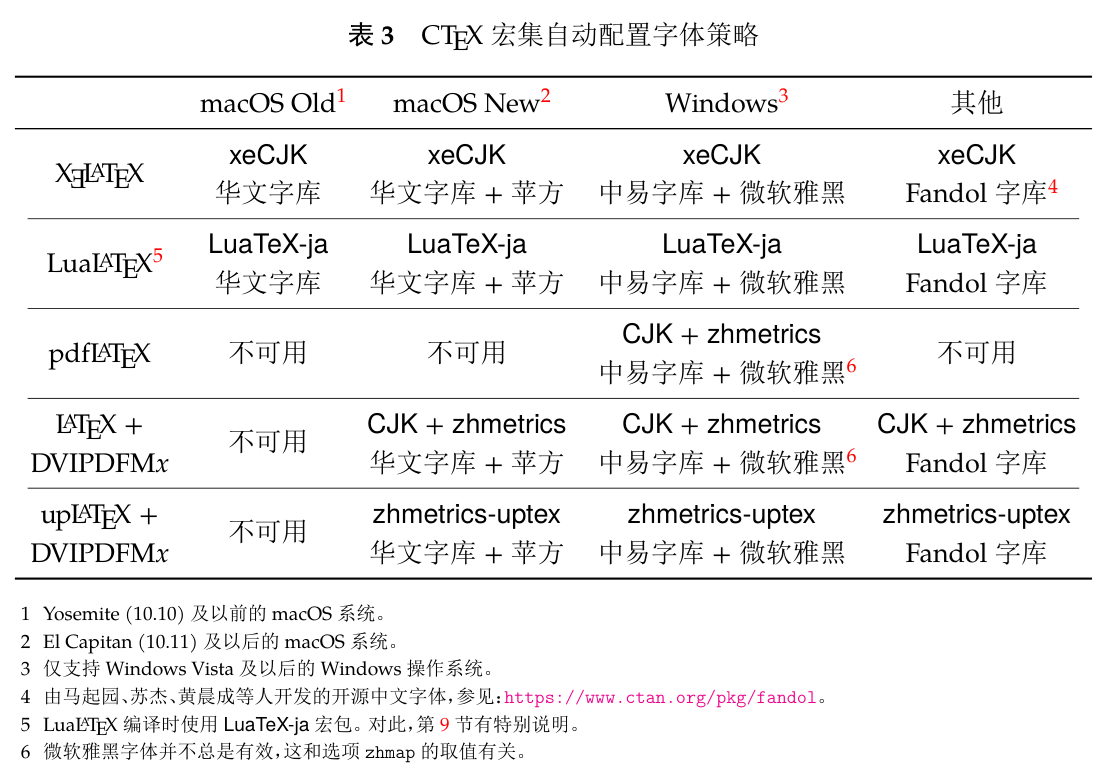
\includegraphics[width=\linewidth]{data/ctex.png}
    \caption{\texttt{ctex}预设包,出自其文档}
\end{figure}

\texttt{ctex}包内有若干套预设好的字体配置,可在导入时使用\texttt{[fontset=X]}选择,\texttt{X}为预设名,详见下表。
\begin{center}
    \begin{longtable}{ccl}
        \textbf{预设名}     & \textbf{使用字体}              & \textbf{版权}                                                   \\
        \hline
        \endfirsthead
        \texttt{adobe}   & Adobe公司的四款中文字体             & 付费商用                                                          \\
        \hline
        \texttt{Fandol}  & Fandol中文字体                 & \stepcounter{footnote} \makecell[l]{GPL+FE协议\footnotemark 开源: \\放入文档中可以随意\\使用\checkmark} \footnotetext{基于此字体改编、修改等所有再创作的字体产品,均必须同样继承GPL+FE协议开源}\\
        \hline
        \texttt{founder} & 方正公司的中文字体                  & \makecell[l]{书宋/黑体/楷体/仿宋                                      \\ 四种为免费商用\checkmark\\ 原则上需要申请一份\\书面授权书} \\
        \hline
        \texttt{mac}     & macOS系统下的字体                & 印刷时存在侵权问题                                                     \\
        \hline
        \texttt{macnew}  & \makecell{ElCapitan或之后的多字重                                                                 \\华文字体和苹方字体} & 见上 \\
        \hline
        \texttt{macold}  & Yosemite或之前的华文字体           & 见上                                                            \\
        \hline
        \texttt{ubuntu}  & \makecell{思源宋体、思源黑体和\TeX                                                                   \\ 发行版自带的文鼎楷体} & 免费商用\checkmark \\
        \hline
        \texttt{windows} & 中易字体和微软雅黑字体                & 付费商用                                                          \\
        \hline
        \caption{\texttt{ctex}字体预设}
    \end{longtable}
\end{center}

\textit{TeXLive}自带字库中包含\textit{Fandol}系列,各平台均可\texttt{[fontset=fandol]}加载全套\textit{Fandol}字体配置,简单达到跨平台统一。但是它只含GB2312内的字符,可能会出现缺字。如果出现这种问题的话,还是只能自行配置字体。

\section{字体名称查询}

首先是寻找字体。代码寻找字体需要使用字体的系统名称,在Windows中,简单的查找系统字体方法是运行\texttt{fc-list}命令。注意\LaTeX 只能找到\LaTeX 内自带的字体和\texttt{C:\textbackslash{}Windows\textbackslash{}Fonts}目录下的字体。因此安装字体时,需要选择\textbf{为所有用户安装}。

可以用系统命令\texttt{fc-list\ \textgreater{}\textgreater{}\ fonts.txt}生成一个字体表文件,包括系统上的可用字体。增加\texttt{:lang-zh}参数可以指定过滤筛选中文字体。注意一些字体虽然使用时是中文,但其字体文件会被识别为日文或韩文,不会出现在结果中。确定\textbf{英文系列名}时,可以用\texttt{fc-list\ \textbar{}\ Select-String\ "系列名"}来筛选字体列表。中文名可能会是乱码,建议只用英文名进行此项操作。

得出的结果中包含字体名,这里使用开源字体\textit{Vollkorn}系列举例。

\texttt{fc-list\ \textbar{}\ Select-String\ "Vollkorn"}得到的结果如下

\begin{lstlisting}[title=\textit{Vollkorn}查询结果]
C:/Windows/fonts/Vollkorn-Medium.otf: Vollkorn,Vollkorn Medium:style=Medium,Regular
C:/Windows/fonts/Vollkorn-Italic.otf: Vollkorn:style=Italic
C:/Windows/fonts/Vollkorn-Bold.otf: Vollkorn:style=Bold
C:/Windows/fonts/Vollkorn-MediumItalic.otf: Vollkorn,Vollkorn Medium:style=Medium Italic,Italic
C:/Windows/fonts/Vollkorn-BoldItalic.otf: Vollkorn:style=Bold Italic
C:/Windows/fonts/Vollkorn-Regular.otf: Vollkorn:style=Regular
C:/Windows/fonts/Vollkorn-SemiboldItalic.otf: Vollkorn,Vollkorn Semibold:style=Semibold Italic,Italic
C:/Windows/fonts/Vollkorn-Semibold.otf: Vollkorn,Vollkorn Semibold:style=Semibold,Regular
\end{lstlisting}

其中\texttt{*.otf:}和\texttt{:style}之间的即为字体在系统里的名称。

对于字体的特殊风格,可以直接以\texttt{字体名\ 风格}作为字体名加载,如\texttt{Vollkorn\ Semibold\ Italic}。

切记区分大小写,有的字体里会是\texttt{SemiBold},有的是\texttt{Semibold}。

注:一些字体名中含有\texttt{-},在打印时会增加转义符显示为\texttt{\textbackslash{}-},使用这些字体时输入\texttt{-}即可。

另外,也可以使用\href{https://fontdrop.info}{FontDrop!\footnote{https://fontdrop.info}}网站解析单个字体文件,获得字体名。解析样例字体\emph{EBGaramondSC12-Regular.otf}时结果如下。

\begin{lstlisting}[title=FontDrop!解析结果]
You see EB Garamond SC
Name: EB Garamond SmallCaps 12 Regular. Style name: 12 Regular. Version 0.016 © Created by Georg Duffner with FontForge 2.0 (http://fontforge.sf.net)
License: Copyright 2010-2013, Georg A. Duffner (<http://www.georgduffner.at/ebgaramond|g.duffner@gmail.com>), 2013 Siva Kalyan This Font Software  
\end{lstlisting}

其中\texttt{You\ see}后的是字体系列名,而\texttt{Name}与\texttt{.\ Style\ name}之间的即为字体本身在系统里的名称(对于风格字体,即为指定时使用的名称)。

\section{外语字符字体配置}

\LaTeX 的字体配置默认是\textbf{只对部分字符生效}的,需要分别配置,混排时可以叠加指定。

我们先说外语字符。\texttt{ctex}包只对中日韩三语起效,其他语言的字符(不止为ASCII,还包括章节符\S 和摄氏度{\songtien℃}等符号)是默认使用基础字体渲染的,只有\texttt{fontspec}包配置的字体才能起效。

\lstinputlisting[style=TeX,caption=配置默认字体]{codes/font-1.tex}

可以设置三种基础类别的字体:

\begin{tightitem}
    \item 主字体\texttt{\textbackslash{}setmainfont}用\texttt{\textbackslash{}rmfamily}调用
    \item 无衬线字体\texttt{\textbackslash{}setsansfont}用\texttt{\textbackslash{}sffamily}调用
    \item 等宽字体\texttt{\textbackslash{}setmonofont}用\texttt{\textbackslash{}ttfamily}调用
\end{tightitem}

一般设个主字体就够了,其他两种字体是默认格式中使用的,自定义格式时反正也要覆盖掉。

用\texttt{\textbackslash{}newfontfamily}配置新的字体。

\lstinputlisting[style=TeX,caption=自定义字体]{codes/font-2.tex}

\LaTeX 默认寻找同系列的字体作为其加粗和斜体,但可以自行进行指定。

\lstinputlisting[style=TeX,caption=指定加粗和斜体]{codes/font-3.tex}

使用非主字体时,只需要输入配置时设定的字体名即可。

\lstinputlisting[style=TeX,caption=使用自定义字体]{codes/font-4.tex}

\subsection{连字(进阶)}

英文衬线字体中存在连字(ligature),通过设计优化某些字符串的显示方式来提升易读性。最经典的三个案例如下(字体为\textit{Vollkorn})。

\begin{minipage}[c][3\baselineskip]{30\ccwd}
    \centering\fontspec{Vollkorn}\Huge fi fl ff
\end{minipage}

\LaTeX 默认载入一部分通用连字(OTF中tag为liga),能提升英文文本的易读性。而一些字体对连字的设计比较充分,还使用了其他的连字tag。通常类别有:clig指上下文连字(contextual),能使手写体中产生连笔;dlig指自由连字(discretionary),会使文字更花俏;hlig指历史连字(historical)能令文字看起来较为复古;rlig标记必需连字(Required),可以实现“将英语字母拼合得到其他字母”,例如ae拼合为æ。

本教程的正文字体启用了历史连字,因此ct,st上面有一笔勾连;启用了自由连字,因此Th上端出现了融合。

\begin{figure}[H]
    \centering
    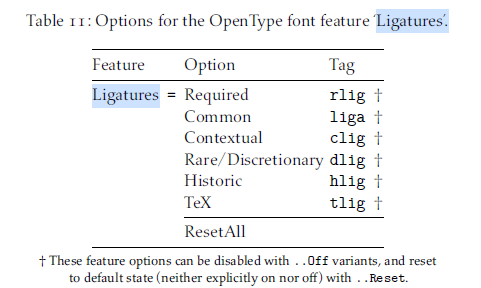
\includegraphics[width=.7\linewidth]{data/ligatures.png}
    \caption{连字配置(出自\texttt{fontspec}包文档)}
\end{figure}

配置时可以添加一个\texttt{[Ligatures=XXX]}参数,启用一些其他tag里的连字,见上图。其中Common是默认打开的。

可以用\href{https://fontdrop.info}{FontDrop!}这个网站来查看字体内连字。有些字体虽然设计了连字,但并没有正确标注,导致这些连字虽然存在但却无法使用。面对这种情况,可以用\href{https://fontforge.org/en-US/}{FontForge\footnote{https://fontforge.org/en-US/}}软件进行\href{https://fontforge.org/docs/tutorial/editexample4.html}{手动标注\footnote{https://fontforge.org/docs/tutorial/editexample4.html}}。

\section{中文字符字体配置}

中文字符,如\texttt{你},\texttt{我},\texttt{;}(中文分号),\texttt{?}(中文问号),均需要使用\texttt{ctex}包内的命令进行字体配置才能正常显示。

如果使用\texttt{ctex}包字库的话,字体命令已经预定义好了。主字体默认为宋体,加粗为黑体,斜体为楷体,等宽(\texttt{\textbackslash{}ttfamily})为仿宋。

\lstinputlisting[style=TeX,caption=\texttt{ctex}默认字体使用方式]{codes/font-7.tex}

如果选择自定义,首先要在引入包时用\texttt{[fontset=none]}避免加载默认字体集,防止产生冲突。

\lstinputlisting[style=TeX,caption=禁用默认中文字体配置]{codes/font-5.tex}

字体配置的命令和\texttt{fontspec}包的差不多,加个\texttt{CJK}即可配置中文、日文、或韩文的字体,配置出的字体只会对这三种语言内的字符生效。

\lstinputlisting[style=TeX,caption=配置中文字体]{codes/font-6.tex}

其中,方正系列四个字体都只有一个字重,而思源两个系列都具有extralight,light,regular,medium,semibold,bold,heavy七个字重,可以进行指定。所有字体中都不含斜体。

\section{字体选用建议}

想看字体效果,先要有一个好使的pdf阅览器。

打印的分辨率是300dpi,而屏幕的分辨率鲜少到达这个级别,屏幕上预览的pdf,精度比起打印机通常是压缩了的。由于渲染机制原因,不同pdf阅览器通常有着不同的压缩效果,建议找一个使用方便,且页面模式下与放大到300dpi下效果最相似的。个人经验中,Windows端的Acrobat DC Pro在英文花体字上发生了笔画显著过细的现象,而SumatraPDF和Edge,Firefox,Chrome均未出现此问题。

\subsection{中文}

中文的可选字体其实不少(\href{https://drxie.github.io/OSFCC/}{开源字体可以见此名单})。我并不大懂字体设计,仅从各方面收集到的资料来看,方正系的字体适用范围最广、知名度最高,设计应该是最佳的。复读,在找方正字体文件时请一定找GBK后缀(书宋为8.87M),而非GB2312或简体后缀(书宋为2.63M)。这样文字比较全。

实际使用时,推荐将方正书宋(书宋即完全针对书籍印刷设计的宋体)作为主字体,指定方正楷体或仿宋作为斜体,以便于在正文中标注少量字符(如引用),这样易读性较佳。

不过,方正书宋只有一个字重免费,固然技术上可以将较粗的思源宋体或方正黑体作为粗体使用,但因为细节差异众多,看起来会很古怪,并不推荐。如果对加粗有明确需求,请挑一款多字重的字体作为主字体。不过,依然可以搭配方正字体作为斜体。

装饰性文字(脚注、页眉页脚等)建议使用方正仿宋或楷体。

各级标题字体建议用不同字重的思源宋体来显示。

思源系列开源,在网上版本很多,不好说谁做了哪些微调。对于一些字体,增加使用\texttt{[CharacterWidth=Full]}这个参数可以调整标点的宽度。

\subsection{外语}

外语的免费字体很多,绝大部分都支持拉丁字母的变体(如é),一部分支持希腊和西里尔字母,选择字体时检查文本所用符号,确认字体可满足即可。在挑花眼的同时,最好也关注一下一些进阶选项,以提升混排效果。这里介绍一些实用的花招,更详细的推荐阅读\texttt{fontspec}包文档。

以下是一些样例,中文使用思源宋体Regular;英文字体均是从网站\href{https://www.1001fonts.com}{1001 Fonts}下载的免费商用字体,全部使用Regular字重的默认配置。

\begin{adjustwidth}{2em}{2em}
    \blankpar

    \songtien 思源宋体\testtext

    \fontspec{Neuton}Neuton\testtext

    \fontspec{EB Garamond 12 Regular}EB Garamond 12 Regular\testtext

    \fontspec{Spectral}Spectral\testtext

    \blankpar
\end{adjustwidth}

思源宋体内置的拉丁字体并不美观,这就是为什么我推荐混排。

\textit{Neuton}的字母偏小。配置时可用\texttt{[Scale=比例]}参数放大。

\textit{EB Garamond}的字母与中文相当契合,但数字采用了与英文相同的三格设计(俗称OldStyle),在数字与汉字混排时看起来会很诡异。可使用\texttt{[Numbers=Lining]}切换到等高数字。注意此方案起效建立在字体中含有等高数字的前提下,不是所有字体都支持。

\textit{Spectral}的字距比起中文明显偏高。可使用\texttt{[LetterSpace=改变数]}来降低字母间距。另,如果想要调整空格宽度,使用\texttt{[WordSpace=空格宽度]}参数即可。

调整后即可达到这样的混排效果。

\begin{adjustwidth}{2em}{2em}
    \blankpar

    \fontspec{Neuton}[Scale=1.1]Neuton\testtext

    \fontspec{EB Garamond 12 Regular}[Numbers=Lining]EB Garamond 12 Regular\testtext

    \fontspec{Spectral}[LetterSpace=-3]Spectral\testtext

    \blankpar
\end{adjustwidth}

不过本质上,\textbf{混排字体的选择取决于文本的字符频}。如果文中存在大量字母(例如ABO中,Alpha/Beta/Omega三个单词会反复出现),那么就应当主要关注字母能否融入正文。

\section{外语字符配置中文字体}

有的中文字体中也一并包含了同风格的外语字符设计。如果需要使用,将其用\texttt{fontspec}包内命令加载,然后叠加使用即可。

\lstinputlisting[style=TeX,caption=中文与外语使用同一字体]{codes/font-8.tex}

这样用很节约找字体的成本,但是不推荐,正如前文所展示的,基本不太可能好看。

\section{字体找不到怎么办?}

第一步,确定字体确实安装在了\texttt{C:\textbackslash{}Windows\textbackslash{}Fonts}文件夹里。

第二步,检查代码中的拼写和\texttt{fc-list}命令获得的一样,特别是大小写。

第三步,在字体名称外面加个中括号。别问为什么,我也不知道,总而言之亲测有效。

\lstinputlisting[style=TeX,caption=找不到字体的处理方案1]{codes/font-9.tex}

第四步,直接配置字体文件名。只要字体装进了默认路径,用这个方法就可以百分百找到。该方案只支持XeTeX和LuaTeX两个引擎,巧了,就是支持中文的两个引擎。

\lstinputlisting[style=TeX,caption=找不到字体的处理方案2]{codes/font-10.tex}

第五步,用\href{https://fontdrop.info}{FontDrop!}网站解析单个字体文件,获得字体名,和\texttt{fc-list}里获得的可能会不一样。

第六步,天涯何处无芳草,字体到处都是,换一个吧。

\chapter{文本导入}

对于已标记好的文本(包括但不限于.docx,.md,.rtf,.epub),用\texttt{pandoc}转化为.tex,然后手动检查一遍即可。如果连\texttt{pandoc}都懒得装,也有很多转化\(\LaTeX\)的网页工具。注意转化会完全继承原文档的格式,大部分时候会有冗余,手动清掉即可。

中文和外语标点存在Unicode码重叠,自动转化工具通常会将标点按外语机制转化,并用外语字体进行渲染,\textbf{需要手动调整单引号}。转化机制不会区分单引号的正反,一律将行首的单引号自动转化为\texttt{\textasciigrave{}}(一个英文反引号),其他单引号转化为\texttt{\textquotesingle{}}(一个英文单引号),因此会出现中文引号不配对的情况。在.tex文件中换回中文单引号即可解决问题。

其他标点的外语化仅会影响外语字体,看不顺眼的话,全文替换换回来即可。

\begin{center}
    \begin{longtable}{ccl}
        \textbf{标点} & \textbf{中文写法} & \textbf{外语写法}                                                                         \\
        \hline
        \endfirsthead
        省略号         & \texttt{……}   & \makecell[l]{\texttt{\textbackslash{}ldots\textbackslash{}ldots},其后可能有\texttt{}(一个空格) \\或\texttt{\{\}}(一组大括号)} \\
        \hline
        左引号         & \texttt{“}    & \texttt{\textasciigrave{}\textasciigrave{}}(两个反引号)                                    \\
        \hline
        右引号         & \texttt{”}    & \texttt{\textquotesingle{}\textquotesingle{}}(两个单引号)                                  \\
        \hline
        破折号         & \texttt{——}   & \texttt{-\/-\/-\/-\/-\/-}(六个“严格来说叫连字符”的减号)                                            \\
        \hline
        \caption{标点中文化}
    \end{longtable}
\end{center}

破折号有点复杂,见后文\emph{\nameref{chsline}}。

\section{\LaTeX 正文语法入门}

对于txt文件,需要手动写一下。\LaTeX 内容写作语法复杂度只在公式上,普通文本只比txt复杂一点点。如果嫌我写得太抽象了,在\textit{Overleaf}上找点模板玩玩即可理解。

\subsection{文件结构}

\LaTeX 文件分导言区和正文区。导言区用于编写预设,正文区用于放置文档内容。

\lstinputlisting[style=TeX,caption=文件结构]{codes/contruct.tex}

导言区的内容在开始制作文档时即全部生效,而正文区的内容在\TeX 编译到此处时才会起效。

\subsection{正文}

正文分段需要使用两个回车(即空一行),连用额外的回车视作无效。

空一段的方法见后文\emph{\nameref{blankpar}}。

单个回车在排版时会视作空格。

用\texttt{\textbackslash{}\textbackslash{}}可以在不换段的情况下换行。

加粗方法:\texttt{\textbackslash{}textbf\{加粗内容\}}

斜体方法:\texttt{\textbackslash{}textit\{斜体内容\}}

\subsection{特殊字符}

如下特殊字符在\LaTeX 中有特殊意义,在正文中使用时不能直接写

百分号(\texttt{\%}),\LaTeX 将其视作注释标志,在正文中使用时请用\texttt{\textbackslash{}\%}。

反斜杠(\texttt{\textbackslash{}},又叫转义符),用处多种多样在正文中使用时请用\texttt{\textbackslash{}textbackslash}。

大括号(\texttt{\{}和\texttt{\}}),默认按分割标记理解在正文中使用时,请用\texttt{\textbackslash{}textbraceleft}和\texttt{\textbackslash{}textbraceright}。

波浪号(\texttt{\textasciitilde{}}),默认按硬空格(不可在此处换行)理解。在正文中使用时,请用\texttt{\textbackslash{}textasciitilde}。

\subsection{标题}

有序标题的标记方法是\texttt{\textbackslash{}级别\{标题内容\}}。序号标记会自动处理,不用写进正文文档区。

无序标题的标记方法是\texttt{\textbackslash{}级别*\{标题内容\}}。不含序号标记,不会参与索引建立。

\section*{}

好了,你入门了。

\chapter{建立文档}

在前文中,你可能已经建立过一些测试文件来研究代码了,在这一节中,我们所讨论的是正经的印刷文档。

\section{文档类型和主字号}

文档类型通常放在文件第一行,较为直观,但不放在那里也行。

\lstinputlisting[style=TeX,caption={文档类型和主字号}]{codes/dclass.tex}

\LaTeX 原生有着\texttt{article}、\texttt{book}、\texttt{report}三种文档类别,对应的\texttt{ctex}类分别为\texttt{ctexart}、\texttt{ctexbook}、\texttt{ctexrep}。三种类别的主要区别在默认层深和排版方式上,虽然排版之后肯定要自己改,但为了直观,本教程推荐使用\texttt{book}类。

\texttt{book}类默认支持三种正文字号10,11,12pt。三种字号可读性都属不错,不建议更大或者更小。如果一定想用其他的,可以使用\texttt{extbook}类文档,支持8,9,10,11,12,14,17,20pt的正文字号。

具体选择时,可以用“磅数÷2.845=毫米数”来计算文字大小。也可参考word,word中的五号字是10.5磅,小四则是12磅。

\texttt{ctex}文档类别除了10,11,12pt外,还支持word款的两种正文字号,配置方法如下

\lstinputlisting[style=TeX,caption={\texttt{ctex}字号}]{codes/fontsize.tex}

\subsection{字号使用}

\begin{figure}[H]
    \centering
    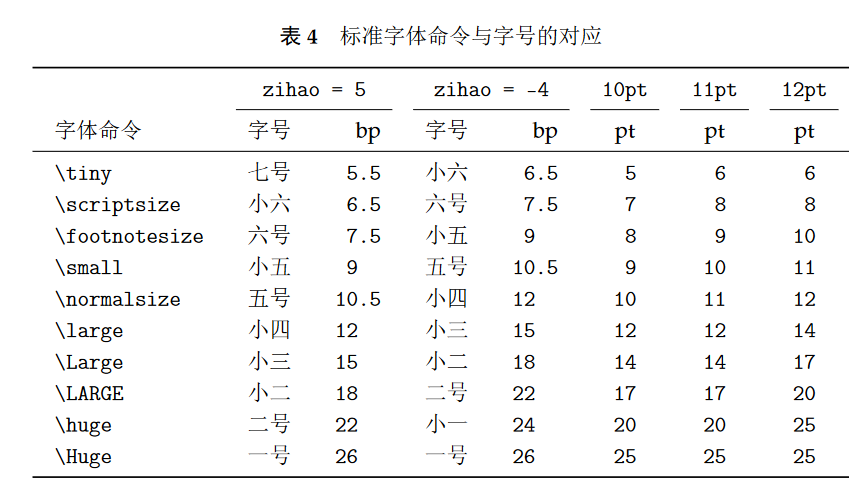
\includegraphics[width=\linewidth]{data/fontsize.png}
    \caption{字号(出自\texttt{ctex}文档)}
\end{figure}

在不同的文档字号时,各个字号命令的对应的字号如上图。

可以用\texttt{\textbackslash{}ctexset\{ziju=额外倍数\}}来额外改变字距,但是不设定的话就是最好看的了。

\section{纸张布局}

一般来说,同人文本的尺寸是A5左右。标准A5是148*210mm,实际中印厂的尺寸不一定能到这里,但我个人还是建议按标准尺寸来做设计,边距留一些余量,印厂不能满足的话再压缩。

\texttt{geometry}是处理布局的包,参数极多,这里只介绍少量常用内容,有其他需求建议阅读文档。

\begin{figure}[H]
    \centering
    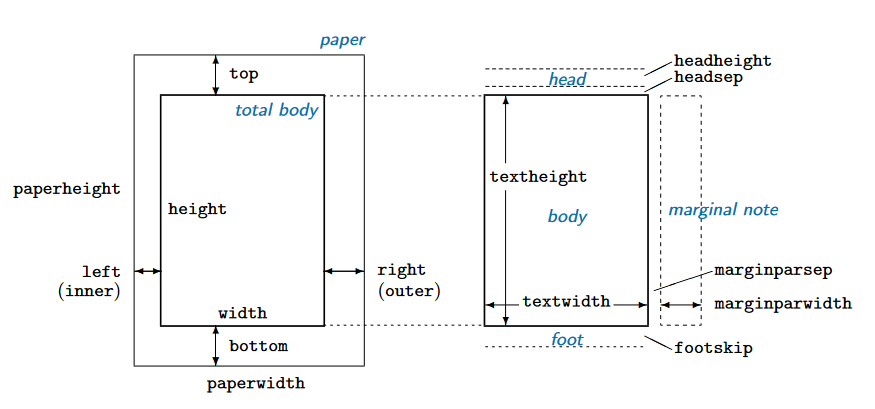
\includegraphics[width=.8\linewidth]{data/paper.png}
    \caption{纸面布局}
\end{figure}

注意水平方向\texttt{left,\ right}和\texttt{inner,\ outer}这两组是单选的关系。双页印刷应当使用\texttt{inner,\ outer}这组参数,能根据页面单双自动调整文字区域位置。

\lstinputlisting[style=TeX,caption={布局}]{codes/geo.tex}

版式规定时,水平竖直方向各三个参数即可,最后一个会自动计算。约束了纸张和版心大小后,内外只定1个就可以了。

\texttt{\textbackslash{}geometry}命令会决定纸张的大小,这点不可修改。边距等版式数值可以在文档内部用\texttt{\textbackslash{}newgeometry}命令进行修改,如

\lstinputlisting[style=TeX,caption={改变布局}]{codes/geotmp.tex}

\subsection{出血}

上述讲解的A5纸张所得到的是效果图,印刷时需要为印厂提供有\texttt{3mm}出血的版本。增加出血很简单,只需要将\texttt{paperwidth,\ paperheight}各增加\texttt{6mm},\textbf{每一处}设置的\texttt{top,\ bottom,\ inner,\ outer,\ left,\ right}各增加\texttt{3mm}即可。\texttt{textwidth}和\texttt{textheight}两个参数不用改变。

\textbf{在正文排版没有bug的情况下},这样的修改可以在效果图四周都增加\texttt{3mm}的白边,中心对齐检阅时,文字位置完全不变。如果修改后有页面发生了移动,那么请在该页的写法上寻找问题。

\section{各级标题}

\texttt{book}类可以使用所有种类的标题,直观地说,可以理解为一本大部头教学书的级别。对于小说,不建议使用超过两级的标题,只选用\texttt{part+chapter}或\texttt{chapter+section}即可。

具体效果如下:

\begin{center}
    \begin{longtable}{ccccl}
        \textbf{层深} & \textbf{标题}                        & \textbf{含义} & \textbf{效果}       & \textbf{用处}           \\
        \hline
        \endfirsthead
        -1          & \texttt{\textbackslash part}       & 部           & \makecell{标题新起一张纸                         \\并独占} & 50+页分割  \\
        \hline
        0           & \texttt{\textbackslash chapter}    & 章           & \makecell{标题新起一张纸                         \\标题下可以有内容} & 15+页分割\\
        \hline
        1           & \texttt{\textbackslash section}    & 节           & 标题与上文同页           & 3\textasciitilde5+页分割 \\
        \hline
        2           & \texttt{\textbackslash subsection} & -           & 标题与上文同页           & 看着用                   \\
        \hline
        3           & \texttt{\textbackslash subsection} & -           & 标题与上文同页           & 看着用                   \\
        \hline
        \caption{各级标题}
    \end{longtable}
\end{center}

新\texttt{part}会重置一部分前文的格式定义,可以通过把命令写进\texttt{part}宏的方式提升复用性。

\lstinputlisting[style=TeX,caption={重载\texttt{part}宏}]{codes/partred.tex}

\section{标题格式}

对于文内标题,使用\texttt{titlesec}包内的命令来配置格式。

对于标题格式,用\texttt{\textbackslash{}titleformat}命令来配置

\lstinputlisting[style=TeX,caption={配置标题格式}]{codes/title-1.tex}

对于标题与上下文的间距,使用\texttt{\textbackslash{}titlespacing}命令

\lstinputlisting[style=TeX,caption={配置标题间距}]{codes/title-2.tex}

标题上的编号默认为\textit{1.1.1}类,即子级编号会带上上级,用以下命令来去除子级的上级编号

\lstinputlisting[style=TeX,caption={编号独立}]{codes/title-3.tex}

\section{换页}

\texttt{\textbackslash{}clearpage}命令可以使后续内容从新的一页上开始,\texttt{\textbackslash{}newpage}则可以新起一栏(单栏模式下即为新开一页)。有浮动要素(如图片、表格)时,二者的处理机制也不同,如需要这部分功能请自行深入研究。

\section{自动空白页}

\texttt{\textbackslash{}chapter}及以上级别的标题会自动新起一张纸。\texttt{book}类文档中默认为双页模式,右页为新纸。当上文结束在奇数页时,会产生一页空白页。不想要的话,可以在定义\texttt{documentclass}的时候增加一个参数\texttt{openany},允许在偶数页开启新内容。

\lstinputlisting[style=TeX,caption={自动空白页}]{codes/page-1.tex}

相对的,如果在使用了\texttt{openany}参数后,希望某页在右页上开始,则可以使用\texttt{\textbackslash{}cleardoublepage}命令。该命令会自动插入空白页,使后续内容从下一个右页铺开。

若希望后文在左页上开始,可以使用以下写法:

\lstinputlisting[style=TeX,caption={左页开始}]{codes/page-2.tex}

\chapter{页面排版}

\section{行高和段距}

首先来明确几个词的含义:

行高:上一行文字底边到这一行文字底边的距离。

行距:即行间距,上一行文字底边到这一行文字顶边的距离。

段距:换段时,在行距基础上额外增加的距离。

段距应为\textbf{行高的整数倍},不然特别的丑。

\subsection{行高}

推荐使用\texttt{\textbackslash{}setspace}包来调整行高。

\lstinputlisting[style=TeX,caption={调整行高}]{codes/spacing.tex}

其中,定义好的三个命令以文字高度(即字号)为基础值,即,单倍行高会使得行高等同于文字高度。但自定义行高的机制则不然。\texttt{\textbackslash{}setstrectch}的基础倍数为\textbf{字号的120\%}。对于10pt的文档字号,\texttt{\textbackslash{}setstrectch\{1\}}会使得行高为12pt,\texttt{\textbackslash{}setstrectch\{1.5\}}会使得行高为18pt。

这些方式都会使\texttt{\textbackslash{}baselineskip}(记录行高的变量)自动跟着变化,可以以此为参数设置缩进。

\subsection{段距}

改变\texttt{\textbackslash{}parskip}即可,默认为0pt。

\lstinputlisting[style=TeX,caption={调整段距}]{codes/parskip.tex}

使用时,最好不要只给一个数,容易导致每页出现大量\texttt{Overfull/Underfull\ \textbackslash{}vbox}错误,解决方法有两种。

\begin{tightenum}
    \item   设置段距时,给出弹性空间。不要让最短段距低于0,会使得段间空白小于行间。
    \item   使用命令允许每页下缘不齐。\textbf{不推荐},在页面布局做不到行对齐时,该命令会使得整体看起来像狗啃的一样。
\end{tightenum}

\lstinputlisting[style=TeX,caption={弹性间距与不对齐}]{codes/flexible.tex}

\section{缩进}

用\texttt{identfirst}包来放开首段的缩进。

\lstinputlisting[style=TeX,caption={首段缩进}]{codes/indent-1.tex}

段首缩进的长度也可以调整,但不是很需要。中文文档用默认的2字宽是最合适的。

\lstinputlisting[style=TeX,caption={修改缩进}]{codes/indent-2.tex}

\section{孤字和孤行(进阶)}

中文排版有一条原则叫“孤字不成行,孤行不成页”。

“孤字不成行”指,一行不能只有一个字(不含标点);“孤行不成页”指一页不能只有一行。很遗憾,这个问题是非常痛苦的“在不同丑里找平衡”大挑战,最省心美观的解法就是放弃。但如果你就不死心,我也可以给你提供一些方案。

(下文中“优雅”的标准是“一,保持内容和格式的分离”,“二,使得不同段落、不同页面的风格尽可能统一”)

\begin{tightitem}
    \item   手动:不优雅,但好使
\end{tightitem}

孤字:把每段最后两个字(以及标点)用\texttt{\textbackslash{}makebox\{\}}括起来。

孤行:引入包\texttt{needspace},在适当的地方加一行\texttt{\textbackslash{}needspace\{高度\}},该代码能使此后一定高度的内容留在同一页上。

评价:后患无穷,只能用于“最终final付梓再也不改了再动我是XX”版本里。更关键的是,我只是说它能解决孤字孤行,没说它会好看。

\begin{tightitem}
    \item   自动:非常优雅,但很难搞
\end{tightitem}

调整单行字数和单页行数,在让排版风格完全没有瑕疵的前提下,通过调参规避孤字和孤行。

评价:可选的参数其实就那些,好消息是可以穷举,坏消息未必举得出来

\begin{tightitem}
    \item   半自动:还算优雅,但不咋好使,与手动或自动搭配或可减轻一些工作量
\end{tightitem}

孤字:\texttt{ctex}包中对于一行内能填充的空白是可规定的,默认为\texttt{1\textbackslash{}ccwd},把这个数改小一些能让标点更加紧凑,部分文本将让一行纳更多的字符,或可避免孤字的出现。支持规定为数(默认单位为\texttt{\textbackslash{}ccwd})或长度。

\lstinputlisting[style=TeX,caption={行伸展量}]{codes/orphan-1.tex}

\texttt{ctex}包中集成了\texttt{CJKpunct}包,可以改变标点风格,把风格改变为开明式(句末全角、句中半角),也能让部分行多容纳一点字符,或可避免孤字。

\lstinputlisting[style=TeX,caption={标点风格}]{codes/orphan-2.tex}

孤行:

拉丁排版中,不希望一个多行段落在一页上只有一行。以下代码会通过调整段距的方法来解决该问题。

\lstinputlisting[style=TeX,caption={孤行}]{codes/orphan-3.tex}

放在中文排版内,它能够解决多行段最后的孤行问题。对于单行段,可能发生“前文占据了更多的垂直空间,使得更多的内容放在了尾页”这样的间接解法。

评价:便于快速感受什么叫“在不同丑里找平衡”

\chapter{引用}

常见的引用基本可以分成两款。

\section{段落格式}

适用于长引用,直接插入正文。

引入\texttt{changepage}包

\lstinputlisting[style=TeX,caption={长引用}]{codes/quote-1.tex}

\section{文本框}

适用于短引用,打包成文本框卡牌,作为浮动对象参与排版。

引入\texttt{minipage}包

\lstinputlisting[style=TeX,caption={短引用}]{codes/quote-2.tex}

默认支持\texttt{htbp}四个位置,\texttt{h}即当前位置(here),\texttt{t}即本页顶部(top),\texttt{b}即本页底部(bottom),\texttt{p}指放在一个仅有浮动对象(图和表)的页面上(page)。四个参数可多选,但优先级固定为\texttt{htbp}。还有一个的\texttt{!}参数,指忽略美学指标。

\chapter{注释}

注释一般是用脚注和尾注两种,视情况自行选择即可。

\section{脚注}

页底脚注以\texttt{\textbackslash{}footnote[编号]\{内容\}}命令来添加。

\lstinputlisting[style=TeX,caption={添加脚注}]{codes/note-0.tex}

引入\texttt{footnpag}包可以在每页重置脚注编号。

\lstinputlisting[style=TeX,caption={每页重置脚注}]{codes/note-1.tex}

脚注高度通常不是整行高,会拉扯当页的行宽,可以用以下代码避免

\lstinputlisting[style=TeX,caption={脚注沉底}]{codes/note-2.tex}

脚注所使用的字体可以自行设定,方法如下

\lstinputlisting[style=TeX,caption={脚注沉底}]{codes/note-3.tex}

使用以下代码令脚注使用罗马数字

\lstinputlisting[style=TeX,caption={脚注罗马数字}]{codes/note-4.tex}

\section{尾注}

建议使用\texttt{endnotes}包来管理尾注。

添加尾注使用\texttt{\textbackslash{}endnote[编号]\{内容\}},在文章任意地方使用\texttt{\textbackslash{}theendnotes}命令输出尾注。第二次使用\texttt{\textbackslash{}theendnotes}会输出第一次输出后新增的尾注。

尾注标题使用以下命令进行修改。

\lstinputlisting[style=TeX,caption={修改尾注标题}]{codes/note-5.tex}

尾注标题默认影响\texttt{\textbackslash{}leftmark}(该命令的用处见页眉页脚一节),可以用以下命令规避。

\lstinputlisting[style=TeX,caption={尾注不改标记}]{codes/note-6.tex}

尾注编号可以用如下代码重置:

\lstinputlisting[style=TeX,caption={重置尾注}]{codes/note-7.tex}

使用以下代码令尾注使用罗马数字

\lstinputlisting[style=TeX,caption={尾注罗马数字}]{codes/note-8.tex}

\chapter{目录}

建议在\textbf{决定了所有内容后},再来设计目录的格式。

用\texttt{\textbackslash{}tableofcontents}命令,在文档中插入目录。

\section{目录标题}

使用如下命令来调整目录页的标题内容,其格式默认与\texttt{\textbackslash{}chapter}级标题相同。\texttt{ctex}文档类别中,目录页标题会翻译为“目录”,也可用如下命令来增加空白间隔。

\lstinputlisting[style=TeX,caption={修改目录页标题}]{codes/toc-1.tex}

\section{目录配置}

用如下命令设置目录层深,层深数值见前文。

\lstinputlisting[style=TeX,caption={设置目录最大层深}]{codes/toc-2.tex}

目录格式配置包并不唯一,我使用的是\texttt{titletoc},配置目录中标题格式的命令是\texttt{\textbackslash{}titlecontents}。

\lstinputlisting[style=TeX,caption={配置目录中标题格式}]{codes/toc-3.tex}

其中,无序号标题默认不出现在目录里,想要的话需要手动添加。可使用以下命令。

\lstinputlisting[style=TeX,caption={手动添加项进目录}]{codes/toc-4.tex}

目录中的标题名默认会显示在序号区和页码区之间,内容默认与正文中的标题名相同,可以不同,有些时候也需要不同。如注只能放在正文中的标题里,而不能出现在目录索引里。

\lstinputlisting[style=TeX,caption={手动添加项进目录}]{codes/toc-5.tex}

\texttt{[目录中的名称]}留空可以使其在目录中以编号节存在,而不显示节名称。

当改变页码字体时,可能会出现\texttt{\textbackslash{}hbox\ underfull}警告,可以用以下代码改变默认的页码宽度。

\lstinputlisting[style=TeX,caption={调整页码宽度}]{codes/toc-6.tex}

\section{局部目录}

\texttt{titletoc}包支持局部目录,用法如下。

\lstinputlisting[style=TeX,caption={局部目录}]{codes/toc-7.tex}

\section{文档内跳转}

虽然是按印刷品的标准的制作,但是为了检阅方便,还是建议使用\texttt{hyperref}包来启用超链接跳转。这样可以从目录直达某个标题。

超链接会带来格式的变化,可以使用一条命令来避免。

\lstinputlisting[style=TeX,caption={超链接}]{codes/toc-8.tex}

\section{页码更改}

在文档中,可以用\texttt{\textbackslash{}setcounter}来修改页码,后续页的页码和目录中的页码都会跟着改变。该命令可以很简便地确定正文首页为第1页。

\lstinputlisting[style=TeX,caption={修改页码}]{codes/pagen-1.tex}

如果某处存在若干页使用其他方式排版(如图文混排时的图片部分),需要将这部分页码空置预留出来,可以使用\texttt{\textbackslash{}addcounter}增加页码。

\lstinputlisting[style=TeX,caption={跳过一些页}]{codes/pagen-2.tex}

\section{目录换页}

可以在正文中手动向目录中增加换页符,确定换页位置。

\lstinputlisting[style=TeX,caption={手动增加换页符}]{codes/toc-8.tex}

\chapter{页眉页脚}

一般使用\texttt{fancyhdr}包来自定义页眉页脚。

\section{页面风格定义}

用\texttt{\textbackslash{}fancypagestyle}命令设计新的页面风格。

\lstinputlisting[style=TeX,caption={定义页面风格}]{codes/hf-1.tex}

位置为\texttt{[L,C,R]}(左中右)和\texttt{[O,E]}(奇偶数)两个选项组成,如\texttt{LE}表示偶数页的左侧,\texttt{C}表示无论奇偶页都显示在中间。

\section{文档自动的标记}

对于\texttt{book}类而言,文档随着进行会自动更新两个标,以便于在页眉页脚中使用。其中\texttt{\textbackslash{}leftmark}记录章标记,\texttt{\textbackslash{}rightmark}记录节标记。如果想要获得部类别的标题和序号,需要自己手动记录。

标记的记录机制与目录中的相同,默认使用正文中的名称,也可专门定义索引名时。

\lstinputlisting[style=TeX,caption={标题索引名}]{codes/hf-2.tex}

\texttt{\textbackslash{}Xmark}默认为\texttt{X\ 序号.\ 索引中的标题名称},可以用重定义的方法来去除章标记中\texttt{X\ 序号.}的部分,节标记同理。

\lstinputlisting[style=TeX,caption={左右标记}]{codes/hf-3.tex}

\LaTeX 中没有预设记录\texttt{part}标题的变量,可以自己设置

\lstinputlisting[style=TeX,caption={\texttt{part}标记}]{codes/hf-4.tex}

也可以在正文中随时使用如下代码来修改左右两种标记。

\lstinputlisting[style=TeX,caption={手动标记}]{codes/hf-5.tex}

左标记默认比右标记高级,所以不能单独定义,不想影响右标记的话填入\texttt{\textbackslash{}rightmark}即可。

\section{页面风格使用}

在文档中使用\texttt{\textbackslash{}pagestyle\{风格名\}}命令设置这一页起的风格。

使用\texttt{\textbackslash{}thispagestyle\{风格名\}}设置当前页的风格,下一页自动还原。

\texttt{fancyhdr}包提供\texttt{fancy},\texttt{plain},\texttt{empty}几种内置风格,\texttt{book}类会自动引用适配不同的页面,可以用上文的定义方法直接重定义。

\texttt{fancy}:页眉外侧角落偶数页为\texttt{\textbackslash{}leftmark},奇数页为\texttt{\textbackslash{}rightmark},页脚中央为\texttt{\textbackslash{}pagenumber}。

\texttt{plain}:页脚中央为\texttt{\textbackslash{}pagenumber}。

\texttt{empty}:什么都没有。

\section{问题处理}

对于由于标题位置而补充的空页,其页面风格默认与前文相同,可以使用引入\texttt{emptypage}包,使得空页面上不显示页眉页脚。

页眉下默认有一条横线,可以用以下命令来设置横线宽度,0为去除。

\lstinputlisting[style=TeX,caption={页眉下横线}]{codes/hf-6.tex}

如果希望页眉页脚溢出在文字区外,可以使用以下写法:

\lstinputlisting[style=TeX,caption={页眉页脚水平溢出}]{codes/hf-7.tex}

\chapter{图片}

处理图片需要的包是\texttt{graphicx}。插入图片的常用代码如下。

\section{插入图片}

\lstinputlisting[style=TeX,caption={插入图片}]{codes/pic-1.tex}

\texttt{figure}的意义是进行内外隔离,为插图服务。对于一些极端情况(如全文档只有图片)可以不包这一层。

\texttt{graphicx}图片位置默认支持\texttt{htbp}四个位置,\texttt{h}即当前位置(here),\texttt{t}即本页顶部(top),\texttt{b}即本页底部(bottom),\texttt{p}指放在一个仅有浮动对象(图和表)的页面上(page)。四个参数可多选,但优先级固定为\texttt{htbp}。还有一个的\texttt{!}参数,指忽略美学指标。如果额外引入\texttt{float}包,那么此处还可使用\texttt{H}作为参数,可以大概理解为“竭尽全力把它放在当前位置”。

导入图片的限制参数有很多,详见文档。最常用的是\texttt{scale=放缩比例}、\texttt{width=图片宽度}、\texttt{height=图片高度},都是等比例放缩。

\section{图片标题}

图片标题用\texttt{caption}这个包来风格化,用法如下。

\lstinputlisting[style=TeX,caption={图片标题}]{codes/pic-2.tex}

\section{旋转}

\texttt{graphics}内置了一个旋转功能,使用方法如下。

\lstinputlisting[style=TeX,caption={旋转}]{codes/pic-3.tex}

顾名思义,就是把内容打包成一个盒子,然后转一下。

\chapter{杂七杂八}

\section{空白页}

空白页要包含若干要素,建议直接写成命令,方便使用。

\lstinputlisting[style=TeX,caption={空白页}]{codes/blankpage.tex}

\section{空白段}
\label{blankpar}

有人(比如我)喜欢用空一段的方式分节。在\LaTeX 中,文字后的空行,不管多少,都视为且只视为一个回车,空一段需要使用如下写法。

\lstinputlisting[style=TeX,caption={空白段}]{codes/blankpar.tex}

\section{规定标点宽度(如中文破折号)}
\label{chsline}

绝大多数中文标点都能在\LaTeX 中按标准方式渲染,但是破折号基本都不会和标准使用方法一样,等同于两个字宽。这与字体和连字均有关系,\href{https://github.com/CTeX-org/ctex-kit/issues/382}{有兴趣可以阅读这篇帖子}。想完美解决很复杂,但是想简单解决真的很简单。

\lstinputlisting[style=TeX,caption={破折号}]{codes/chsline.tex}

使用中,可以将实现方式定义为一个命令,然后把正文中所有破折号替换为该命令,一键解决。

注:\texttt{\textbackslash{}mycommand\hspace{-0.1em}文字}会发生识别错误,应该使用\texttt{\{\textbackslash{}mycommand\}文字}的写法。

\section{特殊字符换字体}

对于个别字符,你可能不满意它的默认字体,(例如问号)。可以用如下写法进行修改。

给它起名\texttt{\textbackslash{}mysymbol},在全文中将中文字符替换成\texttt{\{\textbackslash{}mysymbol\}},大括号防止文字粘连。

设定命令,让\texttt{\textbackslash{}mysymbol}用指定字体渲染。注意大括号需要有两层,限制字体应用范围。

\lstinputlisting[style=TeX,caption={专门字体的符号}]{codes/symbol.tex}

\section{行溢出}

行溢出,即\texttt{Overfull\ \textbackslash{}hbox}警告。一行文字无法恰当地显示在规定的行宽里。

从本质上来说,\textit{警告}并不是一定要消除,因为它不影响功能的实现。但是\LaTeX 中的\textit{警告}与\textit{丑}基本可以画等号,所以排版过程中还是建议解决一下。

调整字号、行宽等基础布局数值,都可能在某些页面产生或消除该警告。

可以增加一个\texttt{sloppypar}域来一劳永逸,即

\lstinputlisting[style=TeX,caption={行溢出的处理}]{codes/ohbox.tex}

但这样的解决方法会导致某一行字距过大,还是影响观感。最美观的解决方法应该是直接调整文本,在确定页面参数后,通过增减这一行的几个字或标点来解决问题。不过因为只能在给自己排版时进行改动,所以大部分时候就只能接受一点点的不美观了。

\section{纸面不充盈}

即\texttt{Underfull\ \textbackslash{}vbox}警告。该警告出现是因为某页前一部分内容不足以填充页面,后一部分内容所需空间又过多,致使页面无法恰当地加载。

调整行宽、行高、段距等基础布局数值,都可能在某些页面产生或消除该警告。

解决方案为在合适的地方进行手动换页(\texttt{\textbackslash{}clearpage}或\texttt{\textbackslash{}newpage})。但由于这样的手动解决方式不是很优雅,所以应当在排版过程的\textbf{最后}进行此调整。

\section{扉页}

虽然可以选择用\texttt{\textbackslash{}maketitle}命令生成一页现成的扉页,但是真的很丑。中文出版物的扉页通常是封面的黑白朴素版,内外呼应,我个人推荐按此办理。根据封面的设计来手动布局,或直接导出一页适于黑白印刷的封面pdf文件(注意出血),插入正文开头作为扉页。

\lstinputlisting[style=TeX,caption={导入扉页}]{codes/titlep.tex}

\section{子文件}

善用子文件可以便于管理,实现格式与内容的分离,以及无关内容彼此分割。

最简单的方法是用\texttt{\textbackslash{}input}命令,将另一个\texttt{.tex}文件引入当前文件,效果相当于用该文件的全部内容替换\texttt{\textbackslash{}input}这一行。

\lstinputlisting[style=TeX,caption={子文件}]{codes/subfile-1.tex}

对于较厚的本,可以使用\texttt{\textbackslash{}subfiles}来分割出子文档,该包可以在不影响整体编译的情况下,独立编译子文档。由于换页的位置会直接影响效果,每个子文档的内容,在主文档中都应当开始于新的一页或新的一张纸。

\lstinputlisting[style=TeX,caption={子文档}]{codes/subfile-2.tex}

对于一些在文档内使用生效的命令,如\texttt{\textbackslash{}pagestyle},需要在子文件的文档内容里和主文件引入子文件前\textbf{都}使用,才能达到相同的渲染效果。

在子文档中,页码自动从1开始。可以手动设置,但不建议这样做,因为手动调整页码的命令在主文件内同样生效,容易产生页码不连续的问题。

\texttt{subfiles}包有时会出现一些bug,如果主文件和子文件渲染出来有页码之外的区别的话,大概就是原生bug造成的。如果调整不出来,可以釜底抽薪,删除开头结尾的\texttt{document}相关声明,改用\texttt{\textbackslash{}input}引入。

\chapter{严格网格排版(进阶)}

严格网格,能让版式像排字印刷时一样精致。

不推荐玩这个,因为哪怕pdf做得再齐,印厂也很可能给你印歪。只是如果你想要一份电子书给自己收藏的话,那它还是很酷的。

\section{行高段距设定}

下文教程将以\texttt{\textbackslash{}baselineskip}(行高)作为纵向的基本单位,所以第一步是将行高调整的命令放到序言区开头。

\lstinputlisting[style=TeX,caption={进阶行高}]{codes/web-1.tex}

段距设定为行高的整倍数,\textbf{不留弹性}。

\lstinputlisting[style=TeX,caption={进阶段距}]{codes/web-2.tex}

\section{版心规划}

可以用\texttt{em}(单字宽度,不考虑字距)或\texttt{\textbackslash{}ccwd}(单字宽度考虑字距)作为单位来定义版心的宽度(\texttt{textwidth}),使得每行严格形成网格。不自行调整字距的话,这两个单位是一样的。

版心高度(\texttt{textheight})应为\texttt{规划行数*行高-行距},\LaTeX 是可以算数的。

\lstinputlisting[style=TeX,caption={进阶版心}]{codes/web-3.tex}

\section{正文对齐}

上面设完之后,纯正文的页面将不会出现任何警告。但各级标题(加上上下留白)的高度几乎不可能是行高的整数倍。

使用现成字号方案的话,由于不同主字号下,各级字号的的大小没什么关系,这里无法给出普适性的精确方案。(需要的话,建议自己算)但可以给非正文区域上下添加弹性空白。如果一页纸上只有正文和单个空白弹性的块,且正文溢出到下页的话,这个做法可以令弹性空白很精确。

\lstinputlisting[style=TeX,caption={进阶弹性空白}]{codes/web-4.tex}

更朴实的方案是把所有非正文用盒子或\texttt{minipage}括起来,固定其所占高度。

\lstinputlisting[style=TeX,caption={进阶标题}]{codes/web-5.tex}

\stopcontents[tutorial]

\listoftables
\listoffigures
\lstlistoflistings

\end{document}